\chapter{Planificación}
\label{chap:planificacionProyecto}
\lettrine{E}{n} este capítulo se propone una planificación del proyecto con el fin de organizar su estructura y exponer sus costes temporales y económicos aproximados necesarios para su realización.

\section{Tareas}
\underline{Tarea 1}. Analizar como está formada la infraestructura, que componentes hardware y software la componen y cual es la función de cada uno de ellos.\\
En cuanto a la parte física se comprueban las especificaciones concretas del hardware de cómputo, almacenamiento y red. También como están organizados y estructurados tanto el sistema de almacenamiento y la red de la infraestructura. En la parte de software, se detallan las funciones de los principales programas y servicios que están instalados en el entorno.\\

\underline{Tarea 2}. Analizar y seleccionar una herramienta de las disponibles en el mercado que se adapte a las necesidades del servicio que se quiere construir y a las características de la infraestructura. La herramienta seleccionada debe permitir reducir el coste y la complejidad de los trabajos de mantenimiento y administración del servicio a la vez que el usuario final lo utiliza de forma sencilla. En este proceso también se debe tener en cuenta la compatibilidad y eficiencia de la nueva herramienta con los componentes ya existentes en el entorno.\\

\underline{Tarea 3}. Tarea que agrupa las tareas dedicadas al proceso de configuración de la infraestructura, configuración de la herramienta seleccionada y su instalación. Estas son las tareas 4, 5, 6, 7, 8, 9 y 10.

\underline{ Tareas 4, 5, 6, 7, 8, 9 y 10.}
Comprobación de requisitos, preparación del entorno, establecimiento de parámetros configuración, despliegue de la plataforma sobre la infraestructura existente y configuración de la plataforma después del despliegue. Antes de realizar la instalación de la nueva herramienta es necesario comprobar sus requisitos necesarios para que las capacidades del servicio final se adapten a las necesidades de uso (tareas 4 y 5). También se deben establecer los parámetros de configuración iniciales que se van a aplicar a la nueva plataforma (tarea 6). Durante el proceso de comprobación de requisitos puede surgir la necesidad de realizar cambios sobre las capacidades de la infraestructura y la configuración de los componentes ya existentes en el entorno inicial para que este se adapte a los requisitos de la nueva plataforma (tareas 7 y 8). Una vez el entorno está preparado para la herramienta pueda ser instalada entonces se efectúa el despliegue (tarea 9), posteriormente se configura y se comprueba el funcionamiento del nuevo servicio (tarea 10).\\

\underline{Tarea 11.} Fin de la instalación y configuración de la plataforma. Marca el final del despliegue y configuración del nuevo servicio en la infraestructura.\\

\underline{Tarea 12}. Diseñar una integración de la nueva plataforma con el sistema de autenticación de la UDC para que los usuarios finales del servicio se puedan autenticar sin necesitar nuevas credenciales. Para ello es preciso comprobar el método de acceso al directorio de usuarios de la UDC y la forma de conectarlo con la plataforma desplegada para, posteriormente, realizar un diseño de la solución. Este proceso requiere realizar una solicitud de acceso a los servicios internos de la UDC.\\

\underline{Tarea 13}. Implementación y despliegue de la integración para la autenticación de usuarios con sus credenciales de la UDC. Durante este proceso puede ser necesario realizar cambios sobre la configuración de perfiles de usuarios que está establecida en la plataforma.\\

\underline{Tarea 14}. Análisis del uso que harán los usuarios del servicio para establecer políticas sobre el uso de recursos. Para realizar este cálculo, primero se debe analizar el uso previo al despliegue del nuevo servicio que los usuarios hacen de la infraestructura y, después, estimar el uso que pueden llegar a realizar una vez el servicio sea accesible. Hay que tener en cuenta la cantidad de usuarios que lo utilizan, que lo van a utilizar y la cantidad de recursos que se emplean y que se van a emplear. Una vez obtenida una estimación, se realiza un diseño de las políticas que se van a aplicar.\\

\underline{Tarea 15}. Diseño de un sistema de facturación/valoración de los recursos del servicio en base a las políticas de uso establecidas. Basándose en las políticas establecidas en la tarea 14, se debe pensar como se pueden aplicar sobre el servicio. Esto puede ser a través de una herramienta externa, en ese caso sería necesario realizar un desarrollo, o integrando la configuración en los parámetros de configuración de la plataforma.\\
La intención de este sistema es limitar la cantidad de recursos que un usuario puede aprovisionar permitiendo aumentar la eficiencia de los recursos físicos reduciendo la cantidad de recursos ociosos.\\

\underline{Tarea 16}. Implementación y despliegue del sistema de facturación/valoración. Para implementar este sistema puede que sea necesario realizar el desarrollo de una herramienta si se determina que no es posible establecerlo a través de los parámetros de configuración de la plataforma. \\

\underline{Tarea 17, 18 y 19}. Recopilación de la información necesaria para la realización de cada tarea. La información de apoyo se debe obtener de documentaciones, artículos, vídeos o libros de  fuentes fiables como empresas desarrolladoras de los productos utilizados o expertos especializados. El objetivo la recopilación de información es obtener conocimiento sobre las herramientas con las que se está trabajando para luego tener una base que facilite la realización de las tareas descritas. Esto se realiza desde el comienzo del proyecto hasta su finalización para tener claros los conceptos que se desarrollan y para conocer los detalles del trabajo que hay que realizar en cada tarea.\\

\underline{Tarea 20, 21 y 22}. Redacción de la memoria del proyecto. Se escribe un documento con todos los detalles de todas las tareas realizadas durante el proyecto, incluyendo los cambios realizados en la infraestructura, las configuraciones establecidas y como se lleva a cabo cada proceso del proyecto. Su objetivo es transmitir el conocimiento adquirido durante el proyecto sobre como realizar el despliegue de una plataforma de virtualización y los beneficios que esta puede tener. La escritura de este documento se realiza a la vez que completa cada tarea para detallar los pasos realizados en cada caso, por lo que su duración es igual a la duración total de todo el proyecto.\\


La duración total del proyecto se estima en 101 días. teniendo en cuenta que el estudiante trabaja durante 4 horas diarias. El coste mostrado se refiere al coste correspondiente al estudiante si trabaja por 25 €/hora. 

\begin{landscape}
\begin{figure}[hp]
  \centering
  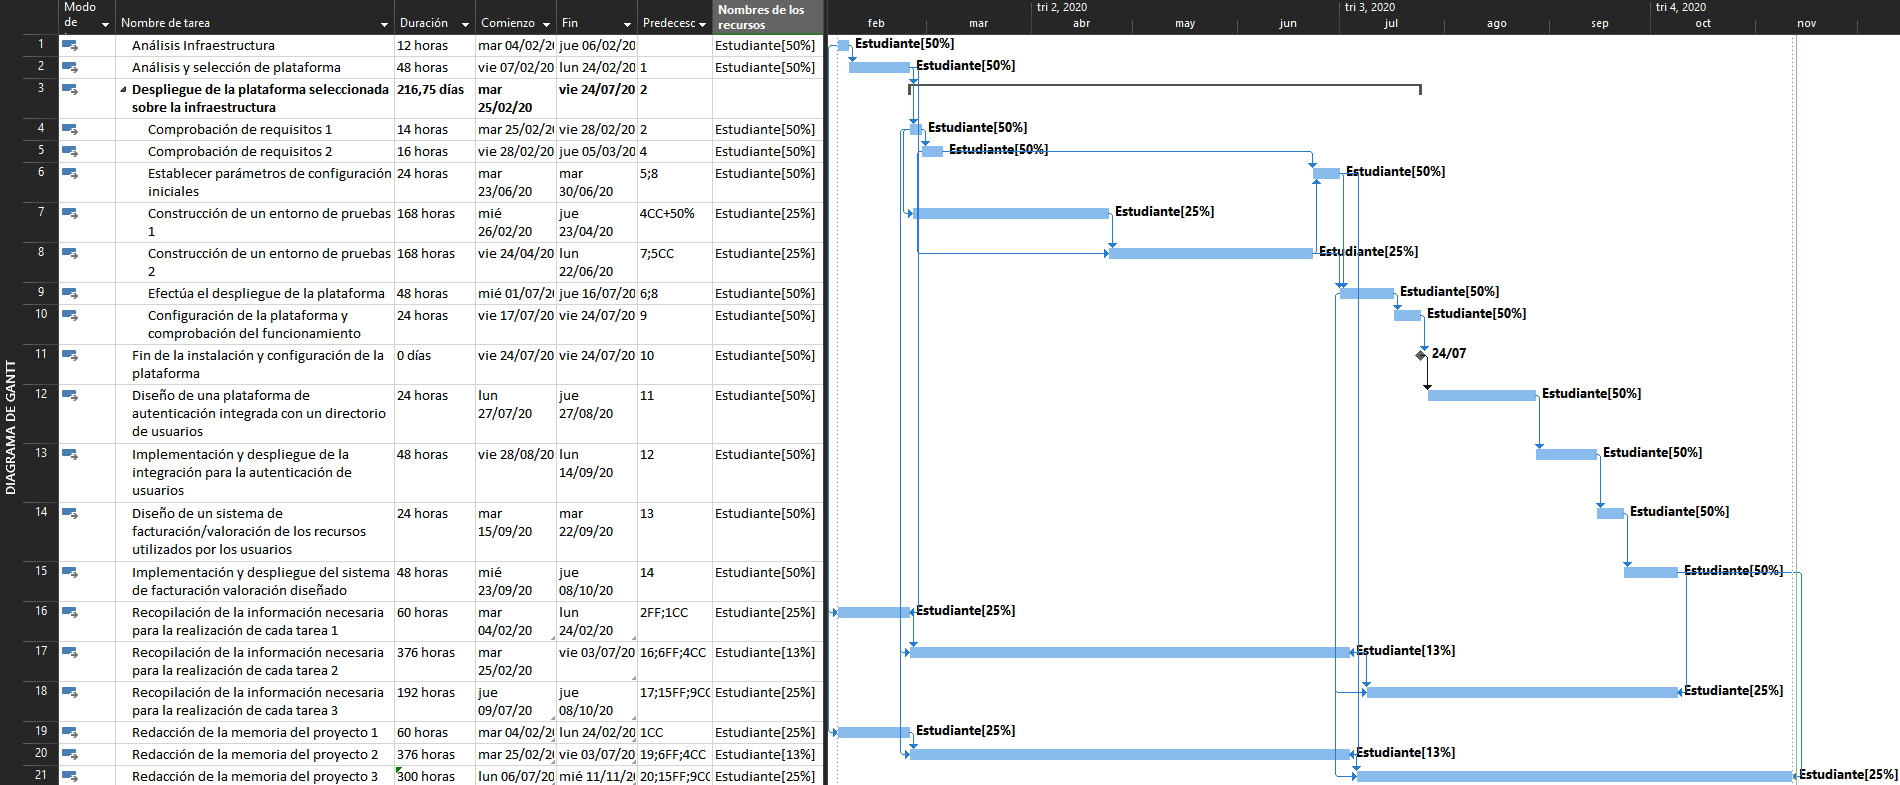
\includegraphics[width=1.5\textwidth]{imaxes/extras/diagramaGranttt.png}
  \caption{Diagrama de Grantt sobre la planificación del proyecto.}
  \label{fig:tareasproyecto}
\end{figure}
\end{landscape}
\begin{figure}[h!]
  \centering
  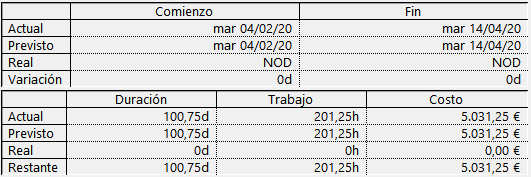
\includegraphics[width=1\textwidth]{imaxes/extras/estadisticasProyecto.png}
  \caption{Estadísticas sobre la planificación del proyecto.}
  \label{fig:estadisticasproyecto}
\end{figure}
\FloatBarrier

\section{Costes}
Los principales costes del proyecto son aquellos relacionados con los trabajadores que lo llevan a cabo y las licencias necesarias para cada componente de VMware Cloud Foundation en la infraestructura\footnote{Los componentes que se especifican son aquellos que son obligatorios para desplegar VMware Cloud Foundation.}.\\
Cada componente de VMware Cloud Foundation requiere su propia licencia\cite{licenses}. Estos componentes son SDDC Manager, VMware vSphere, VMware vCenter, VMware vSAN, VMware NSX for vSphere y VMware vRealize Log Insight. El precio de cada licencia dependerá del número de CPUs físicas sobre las que se va usar esta plataforma por lo que, como en la infraestructura hay un total de ocho hosts con dos CPUs cada uno, \underline{el precio por cada componente} es el siguiente:
\begin{itemize}
    \item \textbf{SDDC Manager}: 18.000€\footnote{Para la edición \textit{Advanced} de VMware Cloud Foundation.} por CPU y 6.500€ anuales de soporte por cada CPU. El precio total de la licencia es de 288.000€ y 104.000€ anuales de soporte por 16 CPUs.
    \item \textbf{VMware vSphere}: 4.000€\footnote{Para la edición \textit{Standard} de VMware vSphere.} por CPU. El precio total de la licencia es de 64.000€ por 16 CPUs y el precio anual por las tareas de soporte es de 16.000€.
    \item \textbf{VMware vCenter}: 6.000€\footnote{Para la edición \textit{Standard} de VMware vCenter} por una licencia que permite usar VMware vCenter sobre todos los hosts del entorno. El precio anual por las tareas de soporte es de 1.500€.
    \item \textbf{VMware vSAN}: 4.000€\footnote{Para la edición \textit{Advanced} de VMware vSAN.} por CPU. El precio total de la licencia es de 64.000€ por 16 CPUs y el precio anual por las tareas de soporte es de 16.000€.
    \item \textbf{VMware NSX for vSphere}: 5.300€\footnote{Para la edición \textit{Advanced} de NSX.} por CPU. El precio total de la licencia es de 84.400€ por 16 CPUs y el precio anual por las tareas de soporte es de 21.100€.
    \item \textbf{VMware vRealize Log Insight}: 1.500€ por CPU. El precio total de la licencia es de 24.000€ por 16 CPUs y el precio anual por las tareas de soporte es de 6.000€.
\end{itemize}

El precio total de todas las licencias necesarias para el entorno, teniendo en cuenta que hay 16 CPUs, sería igual a 530.400€, y el precio total por las tareas de soporte sería igual a 164.600€ anuales.\\

En caso de que ya estén instalados algunos de los componentes entonces solo se requieren licencias para aquellos componentes que aún no están en el entorno. En el caso del entorno inicial, los componentes que ya están instalados son VMware vSphere, VMware vCenter Server. Esto hace que el \underline{coste real para implementar VMware Cloud Foundation} en el entorno sea igual a 460.400€, ya que solo son necesarias licencias para los componentes SDDC Manager, VMware vSAN, VMware NSX for vSphere y VMware vRealize Log Insight. El coste total de la instalación y mantenimiento de la plataforma VMware Cloud Foundation sobre la infraestrructura del CITIC es el siguiente:

    \begin{itemize}
        \item \textbf{Licencias}: 460.400€ en total.
        \item \textbf{Soporte}: 164.600€ anuales.
        \item \textbf{Sueldo empleado}: 5.031,25€ en total.
    \end{itemize}


